\documentclass[12pt]{article}
\usepackage{graphicx}
\usepackage{amssymb}

\usepackage[utf8]{inputenc}
\usepackage{multicol}
\usepackage{listings}
\usepackage{amsmath}
\usepackage{subfig}
\usepackage{float}
\usepackage[left=2cm,right=2cm,top=2cm,bottom=2cm]{geometry}

  
\newlength\tindent
\setlength{\tindent}{\parindent}
\setlength{\parindent}{0pt}
\renewcommand{\indent}{\hspace*{\tindent}}

\DeclareMathOperator*{\argmin}{argmin}
\DeclareMathOperator*{\argmax}{argmax}

\DeclareMathOperator{\tr}{Tr}
\newcommand{\norm}[1]{\left\lVert#1\right\rVert}

\begin{document}

\title{Projet d'imagerie numérique : Inpainting par réseaux \\ \vskip 7px 
\Large Mathis Petrovich et Raphael Bricout
\vskip -2em}
\author{}

\maketitle{}

\section{Introduction}

L'inpainting par réseaux convolutionnels est une application consistant à complèter une image incomplète. Les avancées récentes en deep learning donnent un nouveau souffle à ce processus, en permettant de le traiter d'une manière différente, souvent plus efficace. Cette méthode est encore loin d'être parfaite, mais présente en moyenne de bons résultats, si l'on compare aux méthodes plus traditionnelles. Notre travail consiste ici à analyser les différentes caractéristiques de ce nouveau procédé, à mettre en valeur ses forces et limites, et à essayer de modifier un peu le réseau lui-même pour mieux comprendre son fonctionnement.

\section{Etat de l'art}

L'inpainting n'est pas un problème récent. Il a d'abord été réalisé à
la main pour l'édition de photographies \cite{Staline}. L'arrivée de
l'informatique et du traitement d'images a permit de démocratiser
l'inpainting. Les fondements théoriques sont en grande partie arrivées
à la fin des années 90, puis ont été développées depuis les années
2000. Les techniques utilisées sont diverses. Il est possible
d'utiliser des lignes de niveaux dans le processus, en transformant
l'image à remplir en ligne de niveau, l'inpainter puis revenir en
image. C'est notamment ce qu'utilise \cite{masnou1998}. Les méthodes variationnelles ont également été développées \cite{bertalmio2000}, mais ne fonctionnent pas forcément bien pour les textures. On peut également utiliser des patchs \cite{efros1999}. Cette méthode est plutôt efficace et suite à ce papier de 99, beaucoup d'autres papiers ont vu le jour, comme par exemple Darabi et al.\cite{darabi2012} qui introduit une distance entre les patchs. Cette méthode fonctionne plutôt bien, les textures sont respectées, la complétion est localement cohérente. Le principal problème est qu'on ne peut pas inventer un patch qui n'existe pas dans l'image de test ou dans l'ensemble des images d'entraînement. De plus, les patch trop grands impliquent des problèmes sur les structures et la géométrie qui ne sont pas faciles à résoudes.

Les applications sont diverses : restauration de vieilles photographies et de documents historiques \cite{bertalmio2000}, completion d'objects partiellement obstrués, supression de parasites dans des vidéos \cite{wexler2007}, etc. Plus récemment, on peut utiliser de l'inpainting pour de la reconstitution de surfaces d'objets 3D \cite{bobenko2005} \cite{harary2014}.

\section{Aperçu du papier}

Dans les méthodes exposées plus haut, la complétion est locale, et ne prend donc pas en compte une compréhension globale de l'image. Le principe de ce papier est donc de mixer à la fois une complétion globale et locale.

Ce papier étend le principe d'encodeur de contexte (CE \cite{pathak2016}), qui utilise un réseau convolutionnel adversaire (GAN \cite{goodfellow2014}). Le CE est bien, parce qu'il prend en compte une sémantique, et est donc plus global que les méthodes précédentes. De plus, il permet de créer de nouveaux objets. Cependant, contrairement à la méthode de patchs, mais il n'est pas suffisamment cohérent localement et prends des images de taille fixe.

Le but de ce papier est de garder les avantages de toutes les
méthodes. Il vise à améliorer CE en la rendant localement plus
cohérente, et plus flexible à la taille de l'image. En effet, la
nouvelle architecture est totalement convolutionnelle ce qui permet
d'avoir entrée une image de n'importe quelle taille. \\


\textbf{Remarque} : il eut été intéressant de comparer les résultats du réseau final avec ceux du réseau obtenu uniquement avec en entraînent avec le réseau local et avec le réseau global. Cependant, cela nécessite d'entraîner deux nouveaux réseaux de zéro, ce qui n'est pas possible avec nos moyens.

\section{Fonctionnement du réseau}

\subsection{Structure du réseau}
Sur une échelle globale, le réseau est plutôt simple : 
\begin{itemize}
    \item il y a un réseau de complétion qui à partir d'une image et d'un masque de même dimension, renvoie une image complétée. C'est le réseau principal et lors des tests, il est le seul à être utilisé
    \item le réseau adversaire (GAN) est composé de deux parties qui sont combinées à la fin pour dire si l'image d'entrée est probablement fausse ou non. Les deux parties sont : 
    \begin{itemize}
        \item un discriminateur global, qui va essayer de traquer les erreurs de complétion globales, et donc si le patch complété est cohérent avec toute l'image
        \item un discriminateur local, qui va essayer de déterminer si l'image est localement consistente, et donc si le patch complété est localement cohérent
    \end{itemize}
\end{itemize}

\begin{figure}[H]
    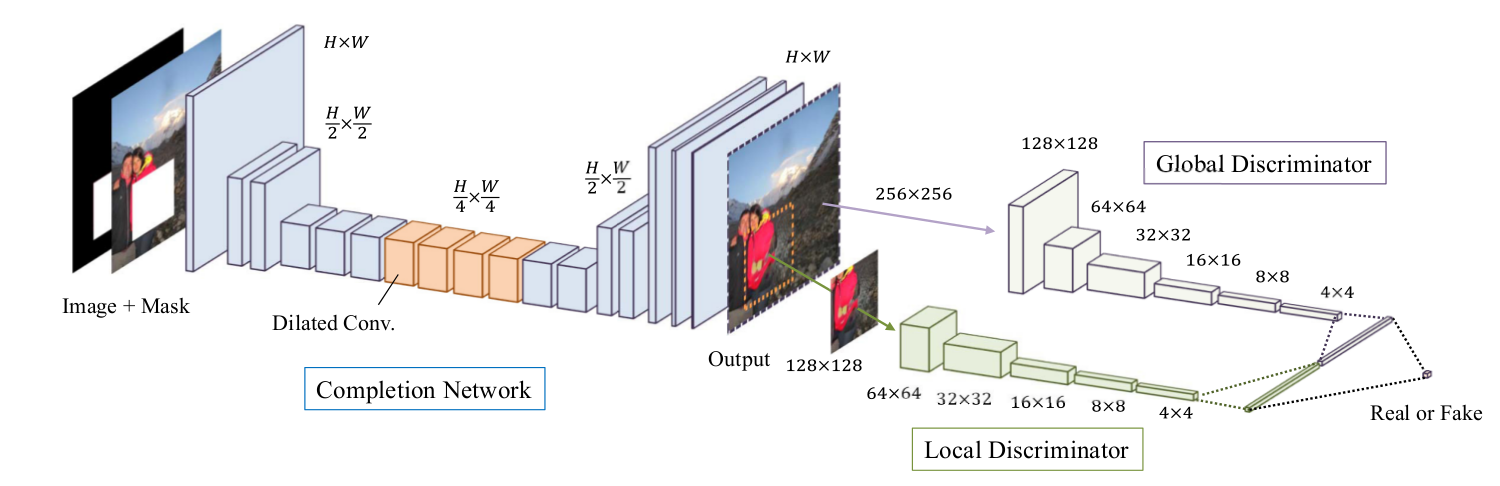
\includegraphics[width=1.0\textwidth]{Images/network_overview.png}
    \caption{Overview of the architecture}
\end{figure}

Pour résumer, on entraîne en parallèle deux réseaux : un qui a pour
but de compléter des images à trous, et un qui doit reconnaître si une
image a été complétée artificiellement. Les deux réseaux sont entraînés mutuellement, le but étant que le réseau qui complète arrive à tromper le réseau qui discrimine.

\subsection{Entrainement}

L'entraînement esst une chose extrêmement délicate pour les GAN de manière générale. Il y a plusieurs problèmes possibles, comme le mod droping par exemple, et il faut entraîner les deux réseaux alternativement, d'une manière qui n'est pas définie de manière théorique, mais qui est plutôt empirique.

\section{Observation sur des exemples}

\subsection{Dataset utilisé pour entrainement : Places2}

Tout d'abord, on peut réutiliser des images appartenant au dataset de validation de Places2. Bien que les images soient diverses, on obtient des résultats corrects pour les images de paysages, même s'ils ne sont pas toujours satisfaisants pour de l'inpainting de visages (cf. section ci-dessous).

\begin{figure}[H]
    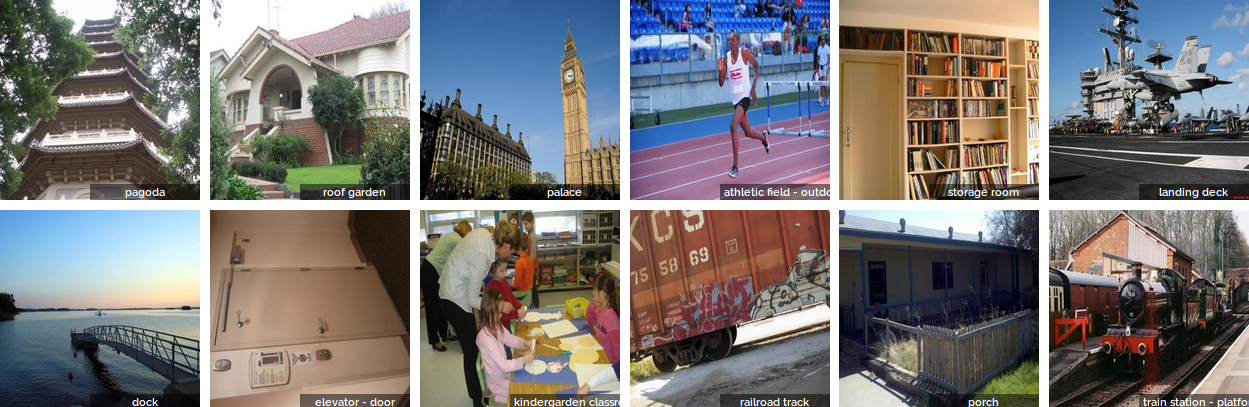
\includegraphics[width=1.0\textwidth]{Images/Places2.png}
    \caption{Randomly chosen images from Places2}
\end{figure}

Les images sont assès diverses, mais si on en regarde un certain nombre, on peut tout de même faire certaines observations : 
\begin{itemize}
\item les images sont naturelles, et tendent à représenter ce qu'un homme peut voir dans la vie
\item les images sont des photos, et non des peintures, des dessins ou des images de synthèse. On s'attend donc à ce que le réseau performe moins bien si on ne donne pas des images de ce style
\item il y a un grand nombre de personnes présentes sur les photos, donc on pourrait s'attendre à ce que les personnes, et notamment les visages soient complétées de manière convainquante.  Ce point sera développé par la suite
\end{itemize}


\subsection{Différentes formes de masques}

L'entraînement du réseau s'est fait en utilisant des masques rectangulaires. Il nous semblait donc possible que l'inpainting sera moins performant si l'on utilise des masques moins réguliers. Pour tester cette hypothèse, nous avons comparé les résultats obtenus sur la même image, en cachant le même objet, mais avec des masques différents.

\begin{figure}[htb]
\centering
  \subfloat{%
    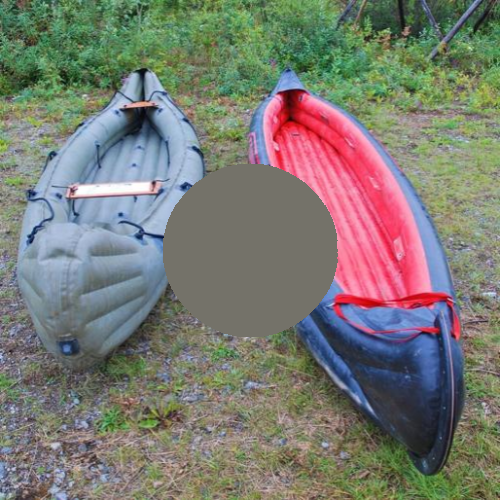
\includegraphics[scale=0.16]{Images/Masks/bateau_in_circle.png}}
  \hfill
  \subfloat{%
    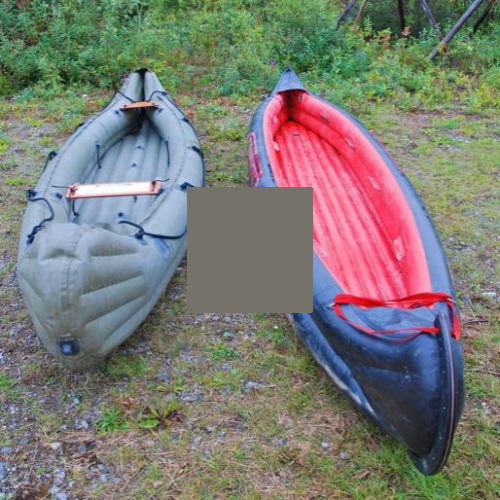
\includegraphics[scale=0.16]{Images/Masks/bateau_in_square.png}}
  \hfill
  \subfloat{%
    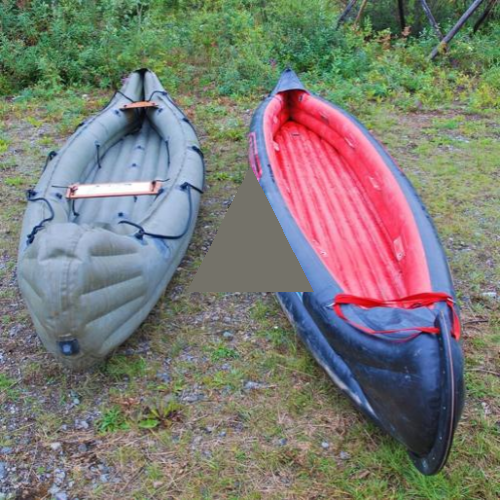
\includegraphics[scale=0.16]{Images/Masks/bateau_in_triangle.png}}
  \hfill
  \subfloat{%
    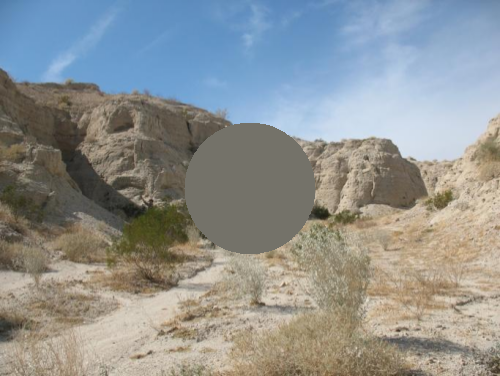
\includegraphics[scale=0.16]{Images/Masks/montagne_in_circle.png}}
  \hfill
  \subfloat{%
    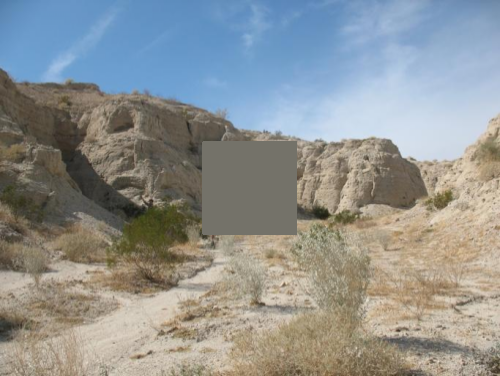
\includegraphics[scale=0.16]{Images/Masks/montagne_in_square.png}}
  \hfill
  \subfloat{%
    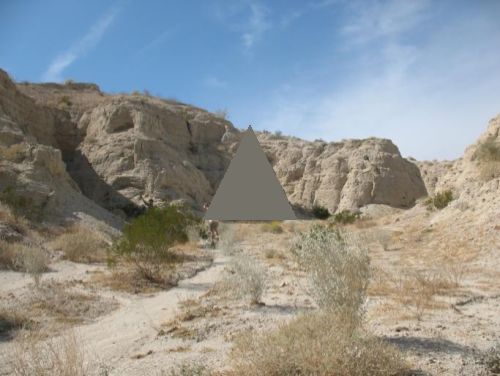
\includegraphics[scale=0.16]{Images/Masks/montagne_in_triangle.png}}
  \hfill
\end{figure}
\begin{figure}[htb]
\centering
  \subfloat{%
    \includegraphics[scale=0.16]{Images/Masks/bateau_out_circle_noise_0_000.png}}
  \hfill
  \subfloat{%
    \includegraphics[scale=0.16]{Images/Masks/bateau_out_square_noise_0_000.png}}
  \hfill
  \subfloat{%
    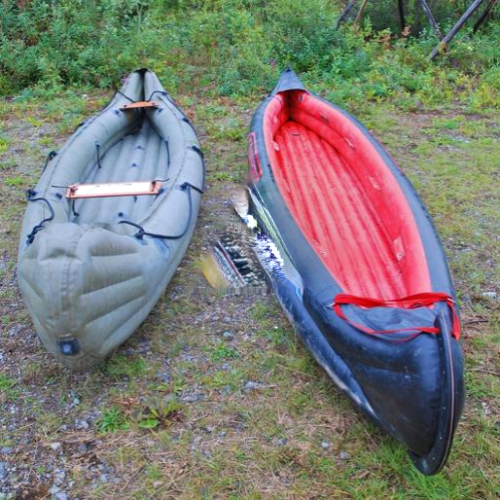
\includegraphics[scale=0.16]{Images/Masks/bateau_out_triangle_noise_0_000.png}}
  \hfill
  \subfloat{%
    \includegraphics[scale=0.16]{Images/Masks/montagne_out_circle_noise_0_000.png}}
  \hfill
  \subfloat{%
    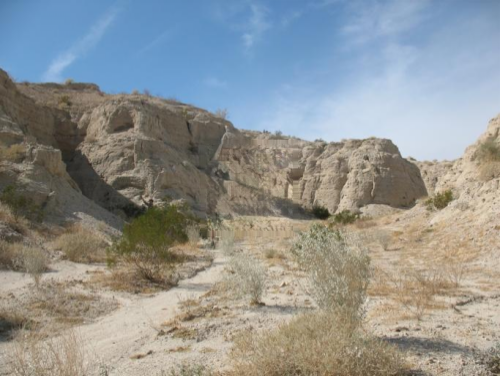
\includegraphics[scale=0.16]{Images/Masks/montagne_out_square_noise_0_000.png}}
  \hfill
  \subfloat{%
    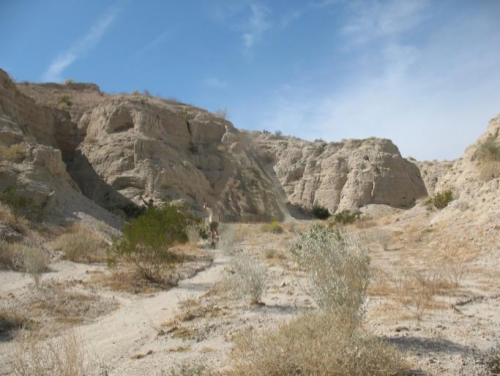
\includegraphics[scale=0.16]{Images/Masks/montagne_out_triangle_noise_0_000.png}}
  \hfill
  \caption{}\label{fig:occlus_dynamic}
\end{figure}

On observe de la surinterprétation plutôt évidente sur la forme du
masque. Quand le masque est carré, comme lors de l'entraînement du
réseau, les résultats sont convainquants. Cependant, les résultats
sont poins bons avec un triangle, et encore pire avec un cercle. On
peut sur les exemples deviner la forme du masque lorsque l'on utilise
autre chose qu'un rectangle. En testant sur d'autres exemples avec des
masques de formes non-géométriques, on obtient des résultats
similaires aux formes non-carrées.

\subsection{Visage (CelebA)}

Un autre point que nous avons voulu tester est l'inpainting sur les visages. En théorie, la méthode utilisant de l'apprentissage profond fonctionne mieux que la mathode par patchs pour compléter des visages, car il est souvent nécessaire d'inventer de nouveaux objets comme des yeux, un nez, des cheveux, etc. et la mathode par patch n'a possiblement pas ces objets en réserve.

\begin{figure}[htb]
\centering
  \subfloat{%
    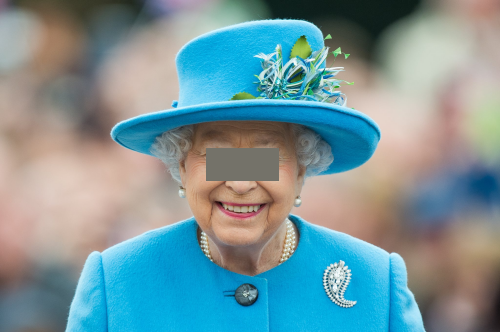
\includegraphics[scale=0.24]{Images/Visages/v_input_1.png}}
  \hfill
  \subfloat{%
    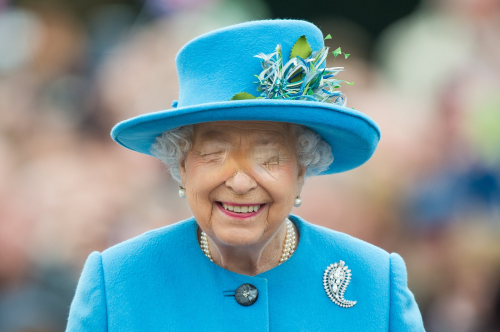
\includegraphics[scale=0.24]{Images/Visages/v_out_1.png}}
  \hfill
  \subfloat{%
    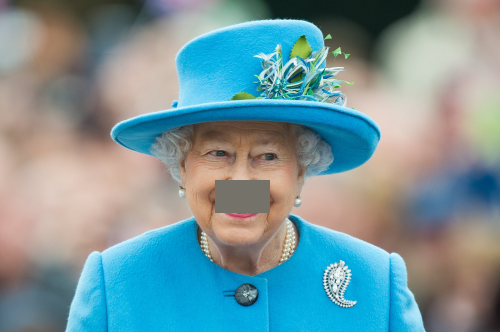
\includegraphics[scale=0.24]{Images/Visages/v_input_2.png}}
  \hfill
  \subfloat{%
    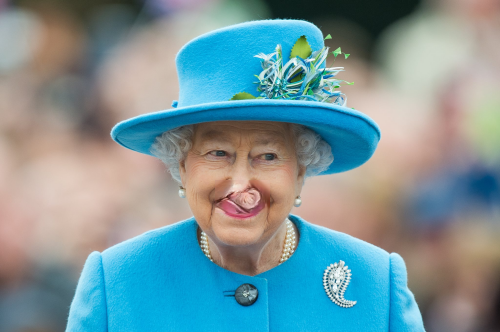
\includegraphics[scale=0.24]{Images/Visages/v_out_2.png}}
  \hfill
  \caption{inputs et outputs (sans postprocess) d'un visage. A gauche, les yeux sont remplaçés par une texture pas très convainquante; à droite, il y a un artefact évident}\label{fig:occlus_dynamic}
\end{figure}

Les tests que nous avons fait (exemple ci-dessus) ne sont pas très
concluant. Le réseau tel quel ne permet pas d'obtenir des résultats
convainquants pour la complétion de visages. En effet, pour obtenir
les résultats présentés dans le papier, le réseau a été entraîné
spécifiquement (finetunning) et nous ne disposons de ces poids pour ce
réseau (non disponible à notre grande déception, malgré une demande sur leur github). Il est cependant légitime de se demander si ledit réseau n'a pas surinterprété les visages au point de les utiliser comme patch pour être capable de les complèter aussi bien que dans l'article.

\subsection{Zero-Padding}

Le papier stipule que les masques qui sont trop près du bord ne donnent pas de bons résultats. Pour vérifier cette affirmation, nous avons effectué plusieurs tests avec des masques plus ou moins près du bord, sur la même image.

\begin{figure}[htb]
\centering
  \subfloat{%
    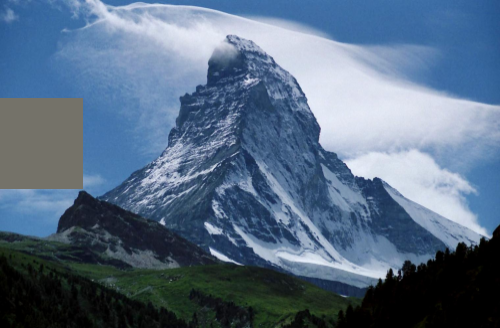
\includegraphics[scale=0.33]{Images/Padding/0_input.png}}
  \hfill
  \subfloat{%
    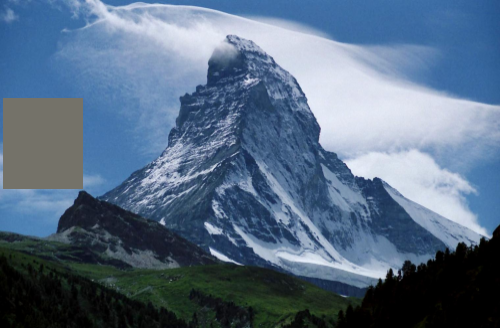
\includegraphics[scale=0.33]{Images/Padding/3_input.png}}
  \hfill
  \subfloat{%
    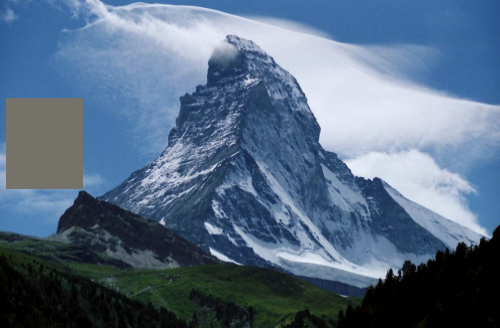
\includegraphics[scale=0.33]{Images/Padding/6_input.png}}
  \hfill
\end{figure}
\begin{figure}[htb]
\centering
  \subfloat{%
    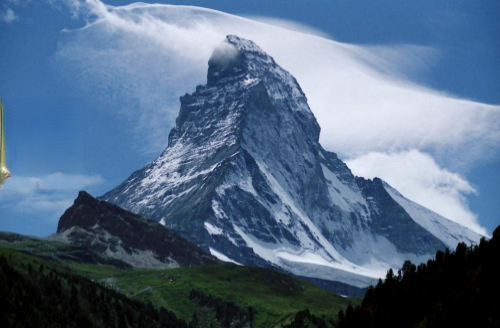
\includegraphics[scale=0.33]{Images/Padding/0_out.png}}
  \hfill
  \subfloat{%
    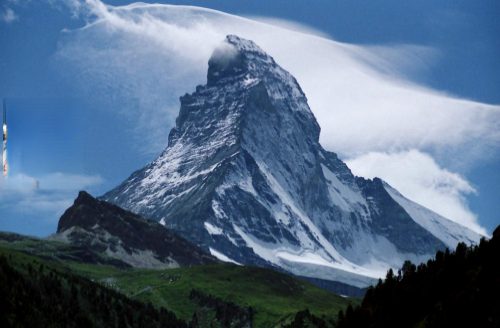
\includegraphics[scale=0.33]{Images/Padding/3_out.png}}
  \hfill
  \subfloat{%
    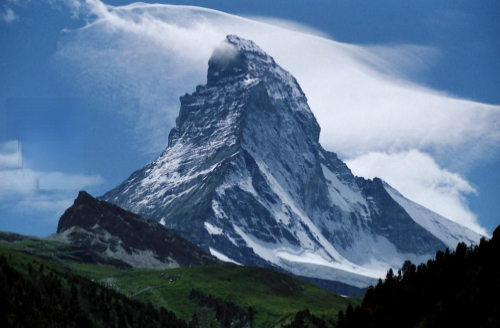
\includegraphics[scale=0.33]{Images/Padding/6_out.png}}
  \hfill
  \caption{inputs et outputs (sans postprocess) à une distance de 0 pixel, 3 pixels, 6 pixels du bord. Seul le dernier cas est convainquant, les autres ont des artefacts évidents}\label{fig:occlus_dynamic}
\end{figure}

Quand le masque est trop près du bord, on constate un artefact dû au fait qu l'on moyenne du noir (en dehors de l'image), ce qui ressort sur le côté. Cependant, dès que l'on est à une distance relativement faible du bord, le résultat n'est plus affecté par ce problème : s'il y a des artefacts, ce n'est plus dû à la trop grande proximité avec le bord.

\section{Modification du réseau}

\subsection{Rajouter du bruit dans les couches}
Pour essayer de comprendre un peu mieux comment fonctionne le réseau,
nous avons rajouter du bruit dans les différentes couches de celui-ci.
Ceci à pour but d'observer l'importance et le rôle de chaque couche dans la
reconstruction (batch normalisation, couches convolutives et couches convolutives dilatées).\\
Nous avons pensé à plusieurs manières d'ajouter du bruit : gaussien et
uniforme. Le bruit gaussien donnant des valeurs trop éloignées de la valeur originale, nous avons choisi d'ajouter du bruit uniforme dépendant des valeurs maximales et minimales de la couche. Les valeurs vont en général de $0$ à $0.5$.\\

\subsubsection{Test avec une image de référence sur les différentes couches}
Pour tenter de distinguer les différentes couches, nous avons lancé un grand nombre de tests sur une seule image, avec le même masque, sur les 33 couches qui composent le réseau, avec $16$ niveaux de bruit. Pour un souci évident de clarté, nous n'en représenteront que certains ici.

\subsubsection*{Sur les couches batch}
\begin{figure}[htb]
\centering
  \subfloat{%
    \includegraphics[scale=0.24]{Images/Batch_norm/02/bateau_in.png}}
  \hfill
  \subfloat{%
    \includegraphics[scale=0.24]{Images/Batch_norm/02/bateau_out_noise_0_00.png}}
  \hfill
  \subfloat{%
    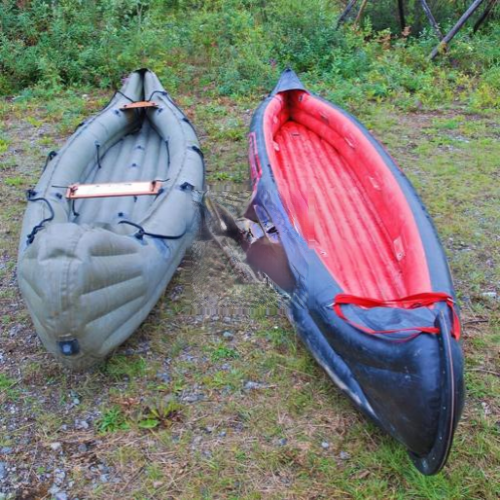
\includegraphics[scale=0.24]{Images/Batch_norm/02/bateau_out_noise_0_14.png}}
  \hfill
  \subfloat{%
    \includegraphics[scale=0.24]{Images/Batch_norm/02/bateau_out_noise_0_28.png}}
  \hfill
\end{figure}
\begin{figure}[htb]
\centering
  \subfloat{%
    \includegraphics[scale=0.24]{Images/Batch_norm/47/bateau_in.png}}
  \hfill
  \subfloat{%
    \includegraphics[scale=0.24]{Images/Batch_norm/47/bateau_out_noise_0_00.png}}
  \hfill
  \subfloat{%
    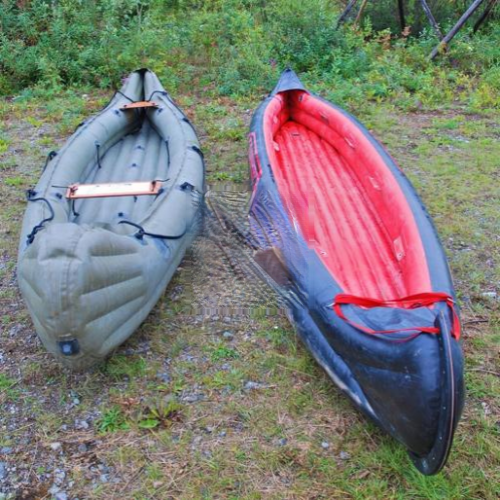
\includegraphics[scale=0.24]{Images/Batch_norm/47/bateau_out_noise_0_14.png}}
  \hfill
  \subfloat{%
    \includegraphics[scale=0.24]{Images/Batch_norm/47/bateau_out_noise_0_28.png}}
  \hfill
  \caption{Exemples de couches de batch normalisation, avec sur la première ligne la couche 2 et sur la deuxième ligne la couche 47. Les bruits sont classés horizontalement : 0, 0.14 et 0.28}\label{fig:occlus_dynamic}
\end{figure}

Sur les couches de batch normalisation, on constate une action plutôt locale, c'est-à-dire que l'on voit les couleurs se propager dans la zone à compléter, mais pas de manière extravagante. On remarque également qu'à cause de la propagation de l'erreur, les premières couches ont beaucoup plus d'impact que les dernières.

\newpage

\subsubsection*{Sur les couches de convolution}
\begin{figure}[htb]
\centering
  \subfloat{%
    \includegraphics[scale=0.24]{Images/Convolution/01/bateau_in.png}}
  \hfill
  \subfloat{%
    \includegraphics[scale=0.24]{Images/Convolution/01/bateau_out_noise_0_00.png}}
  \hfill
  \subfloat{%
    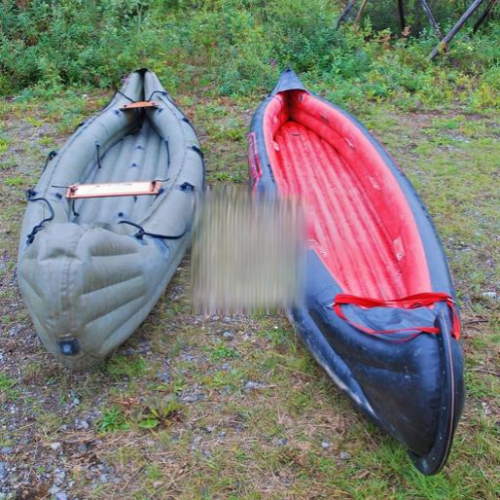
\includegraphics[scale=0.24]{Images/Convolution/01/bateau_out_noise_0_14.png}}
  \hfill
  \subfloat{%
    \includegraphics[scale=0.24]{Images/Convolution/01/bateau_out_noise_0_28.png}}
  \hfill
\end{figure}
\begin{figure}[htb]
\centering
  \subfloat{%
    \includegraphics[scale=0.24]{Images/Convolution/04/bateau_in.png}}
  \hfill
  \subfloat{%
    \includegraphics[scale=0.24]{Images/Convolution/04/bateau_out_noise_0_00.png}}
  \hfill
  \subfloat{%
    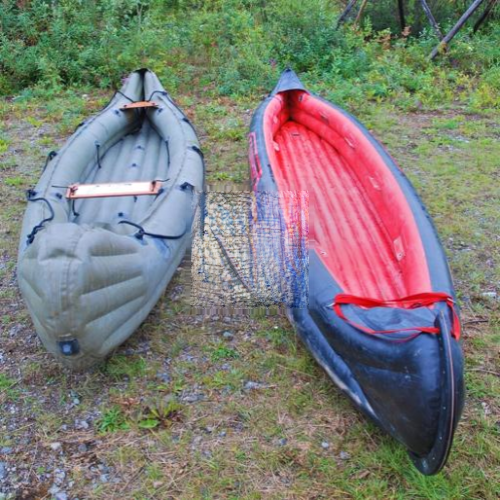
\includegraphics[scale=0.24]{Images/Convolution/04/bateau_out_noise_0_14.png}}
  \hfill
  \subfloat{%
    \includegraphics[scale=0.24]{Images/Convolution/04/bateau_out_noise_0_28.png}}
  \hfill
\end{figure}
\begin{figure}[htb]
\centering
  \subfloat{%
    \includegraphics[scale=0.24]{Images/Convolution/16/bateau_in.png}}
  \hfill
  \subfloat{%
    \includegraphics[scale=0.24]{Images/Convolution/16/bateau_out_noise_0_00.png}}
  \hfill
  \subfloat{%
    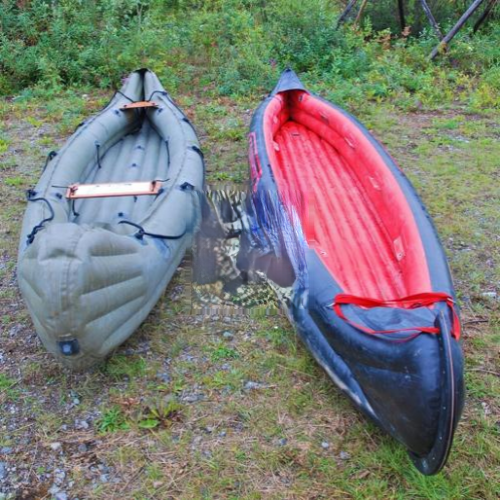
\includegraphics[scale=0.24]{Images/Convolution/16/bateau_out_noise_0_14.png}}
  \hfill
  \subfloat{%
    \includegraphics[scale=0.24]{Images/Convolution/16/bateau_out_noise_0_28.png}}
  \hfill
  \caption{Réponse des couches de convolution avec un bruit. De haut en bas nous avons les couches 1, 4 et 16. De gauche à droite nous avons le masque, et les bruits de 0, 0.14 et 0.28}\label{fig:occlus_dynamic}
\end{figure}

Les couches de convolutions sont plus difficiles à analyser, car elles sont très différentes les unes des autres. Elles possèdent des paramètres différents comme la taille du noyau ou le stride. Nous pouvons cependant observer ce dernier (couche 4) car il a tendance à créer des lignes blanches quand il y a beaucoup de bruit. On observe également parfois du flou, qui vient possiblement du facteur de dilatation (couche 1).\\

On peut faire la même remarque que précédemment à propos de la propagation du bruit.
\newpage
\subsubsection*{Sur les couches de convolution dilatées}
\begin{figure}[htb]
\centering
  \subfloat{%
    \includegraphics[scale=0.24]{Images/Dilated/22/bateau_in.png}}
  \hfill
  \subfloat{%
    \includegraphics[scale=0.24]{Images/Dilated/22/bateau_out_noise_0_00.png}}
  \hfill
  \subfloat{%
    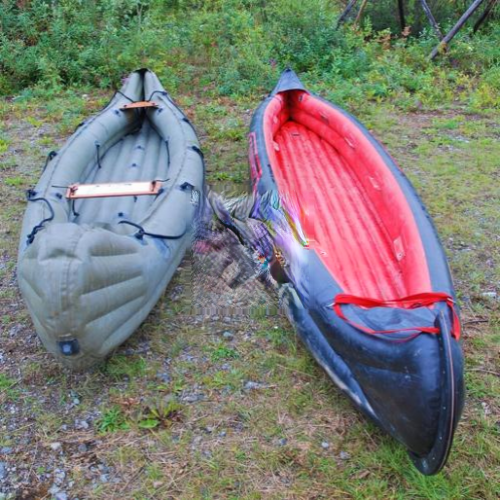
\includegraphics[scale=0.24]{Images/Dilated/22/bateau_out_noise_0_14.png}}
  \hfill
  \subfloat{%
    \includegraphics[scale=0.24]{Images/Dilated/22/bateau_out_noise_0_28.png}}
  \hfill
\end{figure}
\begin{figure}[htb]
\centering
  \subfloat{%
    \includegraphics[scale=0.24]{Images/Dilated/28/bateau_in.png}}
  \hfill
  \subfloat{%
    \includegraphics[scale=0.24]{Images/Dilated/28/bateau_out_noise_0_00.png}}
  \hfill
  \subfloat{%
    \includegraphics[scale=0.24]{Images/Dilated/28/bateau_out_noise_0_14.png}}
  \hfill
  \subfloat{%
    \includegraphics[scale=0.24]{Images/Dilated/28/bateau_out_noise_0_28.png}}
  \hfill
  \caption{Réponse des couches de convolution dilatées avec un bruit. De haut en bas nous avons les couches 22 et 26. De gauche à droite nous avons le masque, et les bruits de 0, 0.14 et 0.28}\label{fig:occlus_dynamic}
\end{figure}

Les couches de convolution dilatées sont difficiles à analyser. On remarque cependant que la complétion n'est absolument pas locale comme on a pu le voir précédemment, ce qui est plutôt rassurant, car il s'agit là du rôle des couches diatées.

\section{Questions additionnelles}

Il y a d'autres questions que nous nous sommes posées, mais il n'est pas possible avec nos moyens d'y répondre. Il est cependant intéressant de se les poser pour avoir une vue plus globale sur le papier.
\begin{itemize}
    \item A quel point le réseau fait-il du surapprentissage lorsque l'on l'entraîne spécifiquement (sur des visages par exemple) ?
    \item Est-ce que la complétion vient d'un "patch" retenu lors de l'entraînement ou bien est-ce qu'elle est créée ?
\end{itemize}



\section{Implementation}

\subsection{Matériel utilisé}
Pour pouvoir faire autant de test, nous avons utilisé un GPU (Titan X
Pascal). Ceci à eu pour effet d'accelerer l'impainting d'un facteur 20
($30s$ sur GPU à $1,5s$ sur CPU pour inpaint une image).

\subsection{Créateur de masques}
Pour pourvoir faire des tests plus rapidement, nous avons développé
un programme qui nous permet d'éditer un masque facilement.
Il permet de:
\begin{itemize}
\item Créer un masque
\item Changer la forme du "pinceau" (carré/cercle)
\item Changer le rayon/côté de la forme
\item Mode édition et mode suppresion
\item Sauvegarder le masque
\end{itemize}

\begin{figure}[htb]
\centering
  \includegraphics[scale=0.50]{Images/editor.png}
  \caption{Capture d'écran du programme}
\end{figure}

\subsection{Code}
Nous avons au début fait des tests "à la main" en modifiant les fichiers
lua de l'article.

Puis nous avons rajouter des paramètres proprement pour pouvoir
l'interfacer avec du code python.

En effet, python dispose de beaucoup de fonctions utile pour gérer les
fichiers (avec le module os) et permet de lancer le code lua.


Nous avons crée des masques algorithmiquement (carré,
cercle ou triangle) centré au milieu de l'image ayant pour dimension
$min(width, height)/4$.

\subsection{Statistiques}
Nous avons tester pour chaque couche (environ 50), plusieurs niveaux de
bruit (10), plusieurs formes (3) et plusieurs images (10). Ce qui fait
que nous avons impainté plus de $15000$ images (ce qui fait environ 2Go) 



\newpage

\section{Bonus}

\subsection{Test du réseau sur des images non naturelles}

\subsubsection*{Avec un style un peu différent}
\begin{figure}[htb]
\centering
  \subfloat{%
    \includegraphics[scale=0.24]{Images/CoL/input_1.png}}
  \hfill
  \subfloat{%
    \includegraphics[scale=0.24]{Images/CoL/input_2.png}}
  \hfill
  \subfloat{%
    \includegraphics[scale=0.24]{Images/CoL/input_3.png}}
  \hfill
  \subfloat{%
    \includegraphics[scale=0.24]{Images/CoL/input_4.png}}
  \hfill
\end{figure}
\begin{figure}[htb]
\centering
  \subfloat{%
    \includegraphics[scale=0.24]{Images/CoL/out_1.png}}
  \hfill
  \subfloat{%
    \includegraphics[scale=0.24]{Images/CoL/out_2.png}}
  \hfill
  \subfloat{%
    \includegraphics[scale=0.24]{Images/CoL/out_3.png}}
  \hfill
  \subfloat{%
    \includegraphics[scale=0.24]{Images/CoL/out_4.png}}
  \hfill
  \caption{inputs et outputs (sans postprocess) sur une image ayant un style particulier (type pastel).}\label{fig:occlus_dynamic}
\end{figure}

Sur un style qui diffère un peu, mais pas de manière trop brutale avec les images naturelles qui composent en immense majorité Places2 (il n'est pas exclu qu'il y ait des images de pastels), on obtient un résultat qui contient parfois des artefacts, mais qui est parfois convainquant, ce qui est plutôt une bonne surprise.

\subsubsection*{Avec un style très particulier}
\begin{figure}[htb]
\centering
  \subfloat{%
    \includegraphics[scale=0.33]{Images/Gogh/input_1.png}}
  \hfill
  \subfloat{%
    \includegraphics[scale=0.33]{Images/Gogh/input_2.png}}
  \hfill
  \subfloat{%
    \includegraphics[scale=0.33]{Images/Gogh/input_3.png}}
  \hfill
\end{figure}
\begin{figure}[htb]
\centering
  \subfloat{%
    \includegraphics[scale=0.33]{Images/Gogh/out_1.png}}
  \hfill
  \subfloat{%
    \includegraphics[scale=0.33]{Images/Gogh/out_2.png}}
  \hfill
  \subfloat{%
    \includegraphics[scale=0.33]{Images/Gogh/out_3.png}}
  \hfill
  \caption{inpainting (sans postprocess) de la nuit étoilée de Van Gogh}\label{fig:occlus_dynamic}
\end{figure}


Comme on pouvait s'y attendre, le réseau à beaucoup de mal à s'adapter au style d'une image particulière. La complétion n'est pas abérrente en soi (localement), mais elle ne s'accorde pas avec le style global de l'image.

\newpage

\bibliographystyle{plain}
\bibliography{bib}

\end{document}
